%KECReportFormat.tex
%%%%%%%%%%%%%%%%%%%%%%%%%%%%%%%%%%%%%%%%%%%%%%%%%%%%%%%%%%%%%%%%%%%%%%%%%%%
%DO NOT MAKE CHANGES IN THIS FILE

\documentclass[12pt, a4paper]{report}
\usepackage[left = 1.5in, right = 1in, top = 1in, bottom = 1in]{geometry}%for margin
\usepackage{amsfonts, amsmath, amssymb} %for mathematical equations
\usepackage{graphicx} %for images
\usepackage{times} %font Times New Roman Font
\usepackage{float} %required if you use H(strictly here) position for floats
\usepackage[skip = 8pt,tableposition=top, figureposition=bottom]{caption}%adjust spacing of captions and specify where captions are
\usepackage{hyperref} % for easy Navigation in document, also puts links in TOC, LOF, LOT...
\usepackage{setspace} %to change line spacing in some portion \singlespacing \onehalfspacing \doublespacing
\usepackage{acro} %for List of Abbrreviation and Symbol
\acsetup{first-style = short} % set to display only short form on the command \ac{}

%packages required for complex tables
\usepackage{bigstrut} 
\usepackage{multirow}

\renewcommand{\contentsname}{Table of Contents} %Change TOC Heading ... default is "Contents" 

\parindent 0pt	%removes the indent in paragraph
\setlength{\parskip}{18pt}	%for paragraph spacing
\renewcommand{\baselinestretch}{1.5}   %Line Spacing = 1.5 line-spaces

%to reduce spacing in sections
\usepackage{titlesec}
\titlespacing*{\section}{0pt}{0pt}{0pt} %left, top, bottom spacings
\titlespacing*{\subsection}{0pt}{0pt}{0pt}
\titlespacing*{\subsubsection}{0pt}{0pt}{0pt}
\titlespacing*{\paragraph}{0pt}{0pt}{0pt}
\titlespacing*{\subparagraph}{0pt}{0pt}{0pt}

%adjust fontsizes\ of sections
\titleformat*{\section}{\fontsize{14pt}{18pt}\bfseries}
\titleformat*{\subsection}{\fontsize{13pt}{18pt}\bfseries}
\titleformat*{\subsubsection}{\fontsize{12pt}{18pt}\bfseries}
\titleformat*{\paragraph}{\fontsize{12pt}{18pt}\bfseries}
\titleformat*{\subparagraph}{\fontsize{12pt}{18pt}\bfseries}

%to reduce separation between points in list
\usepackage{enumitem}
\setlist[enumerate]{nosep} % no separation between items in enumerate
\setlist[itemize]{nosep} % no separation between items in itemize
%use \vspace{-18pt} before list to reduce paragraph spacing between list and preceeding paragraph.

%Changes for Chapter Heading Spacing and formats for numbered chapters
\makeatletter
\def\@makechapterhead#1{%
  %\vspace*{50pt}%
  {  \MakeUppercase{\ifnum \c@secnumdepth >\m@ne
        \fontsize{16pt}{1}\bfseries \@chapapp \space \thechapter\vspace{5pt}\\
    \fi
    \interlinepenalty\@M
     \bfseries #1}\par\nobreak
    %\vskip 0pt
  }}
\makeatother

%%%%%%%%%%%%%%%%%%%%%%%%%%%%%%%%%%%%%%%%%%%%%%%%%%%%%%%%%%%
%to adjust Heading spacings and fonts For unnumbered chapters, TOC, LOF ...
\makeatletter
% Redefine the \chapter* header macro to remove vertical space
\def\@makeschapterhead#1{%
  %\vspace*{50\p@}% Remove the vertical space
  {\newpage \parindent \z@ \raggedright
    \normalfont
    \interlinepenalty\@M
    \center \fontsize{16pt}{1} \bfseries \MakeUppercase{#1}\par\nobreak
    %\vskip 18\p@ % adjust space after heading 18pt
  }}
\makeatother 
%%%%%%%%%%%%%%%%%%%%%%%%%%%%%%%%%%%%%%%%%%%%%%%%%%%%%%%%%%%

%%%%%%%%%%%%%%%%%%%%%%%%%%%%%%%%%%%%%%%%%%%%%%%%%%%%%%%%%%%%%%%%%%%%%%%%%%%
% newcommand for generating Cover Page
\newcommand{\KECcoverpage}
{
\begin{titlepage}
\begin{center}
\Large{\textbf{KANTIPUR ENGINEERING COLLEGE}}\\
\large{\textbf{(Affiliated to Tribhuvan University)}}\\
\large{\textbf{Dhapakhel, Lalitpur}}\\
\vfill	%vertically fill the space 
\begin{figure}[h] % h: put logo "here"
\begin{center}

\includegraphics[width=25mm, height = 25mm]{images/logo.png}
\end{center}
\end{figure}

\large{\textbf{[Subject Code: \subCode]}}\\ %Change This Line
\large{\textbf{A \MakeUppercase{\project} \MakeUppercase{\doc} ON}}\\ %Change This Line
\Large{\textbf{\MakeUppercase{\projectTitle}}}\\

\vfill	%vertically fill the space 
\large{\textbf{Submitted by:}}\\
\large{\textbf{\submittedBy}}\\
\vfill	%vertically fill the space 
\textbf{A \MakeUppercase{\project} SUBMITTED IN PARTIAL FULFILLMENT OF THE REQUIREMENT FOR THE DEGREE OF \MakeUppercase{\degree}}\\

\vfill	%vertically fill the space 
\large{\textbf{Submitted to:}}\\
\large{\textbf{\submittedTo}}\\
\vfill
\large{\textbf{\defMonth, \defYear}}
\pagebreak
\end{center}
\end{titlepage}
}
%%%%%%%%%%%%%%%%%%%%%%%%%%%%%%%%%%%%%%%%%%%%%%%%%%%%%%%%%%%%%%%%%%%%%%%
% newcommand for generating Cover Page
%Title Page
\newcommand{\KECtitlepage}
{
\begin{titlepage}
\begin{center}
\Large{\textbf{\MakeUppercase{\projectTitle}}}\\

\vfill	%vertically fill the space 

\large{\textbf{Submitted by:}}\\
\large{\textbf{\submittedBy}}\\


\ifhassupervisor % Displays Supervisor name only if \hassupervisortrue
	\vfill	%vertically fill the space 
	\large{\textbf{Supervised by:}}\\
	\large{\textbf{\supervisor}}\\
	\large{\textbf{\degSup}}\\
\fi

\vfill	%vertically fill the space 
\textbf{A \MakeUppercase{\project} SUBMITTED IN PARTIAL FULFILLMENT OF THE REQUIREMENT FOR THE DEGREE OF \MakeUppercase{\degree}}\\

\vfill	%vertically fill the space 
\large{\textbf{Submitted to:}}\\
\large{\textbf{\submittedTo}}\\
\large{\textbf{Kantipur Engineering College}}\\
\large{\textbf{Dhapakhel, Lalitpur}}\\

\vfill
\large{\textbf{\defMonth, \defYear}}
\thispagestyle{empty}\\ %to remove page number
\pagebreak
\end{center}
\end{titlepage}
}
%%%%%%%%%%%%%%%%%%%%%%%%%%%%%%%%%%%%%%%%%%%%%%%%%%%%%%%%%%%%%%%%%%%%%%
%command for copyright page
\newcommand{\KECcopyright}
{
\chapter*{Copyright}%Required only for Final Defense of Major Project
\addcontentsline{toc}{chapter}{Copyright}
The author has agreed that the library, Kantipur Engineering Collage, may make this report freely available for inspection. Moreover the author has agreed that permission for extensive copying of this report for scholarly purpose may be granted by the supervisor(s), who supervised the project work recorded herein or, in their absence, by the Head of the Department wherein this project was done. It is understood that due recognition will be given to the author of this report and to the \submittedTo, Kantipur Engineering College in any use of the material of this report. Copying or publication or other use of this report for financial gain without approval of the \submittedTo, Kantipur Engineering College and author’s written permission is prohibited.\par Request for permission to copy or to make any other use of the material in this report in whole or in part should be addressed to:

Head\\
\submittedTo\\
Kantipur Engineering College\\
Dhapakhel, Lalitpur\\
Nepal
}
%%%%%%%%%%%%%%%%%%%%%%%%%%%%%%%%%%%%%%%%%%%%%%%%%%%%%%%%%%%%%%%%%%%%%%
%command for Approval Letter
\newcommand{\KECapproval}
{
\chapter*{Kantipur Engineering College
\vskip -10pt}%Required only for Final Defense of Major Project
\begin{center}
\fontsize{12.8pt}{1} %size decreaced to adjust department name in single line
\textbf{
\MakeUppercase{\submittedTo}\\ %for department name
}
\vskip 10pt
\fontsize{16pt}{1}
\textbf{APPROVAL LETTER}
\end{center}
\vskip -16pt
\addcontentsline{toc}{chapter}{Approval Letter}%
The undersigned certify that they have read and recommended to the Institute of Engineering for acceptance, a project report entitled "\projectTitle " submitted by \\
\submittedBy \\
in partial fulfillment for the degree of \degree. \par
{\vspace{25pt}
..........................................\\
Supervisor\\
\supervisor \\
\degSup\\
\vspace{25pt}\\
..........................................\\
External Examiner\\
\external\\
\degExternal\\
\vspace{25pt}\\
..........................................\\
\hod\\
Head of Department\\
\submittedTo
\vspace{10pt}\\
Date: \defMonth\space\defDay ,\space \defYear
\singlespacing\par
} %single spacing for the texts inside {}
}

%command for list of abbreviations
\newcommand{\KECloa}
{
\chapter*{List of Abbreviations}
\addcontentsline{toc}{chapter}{List of Abbreviations}
\vskip -42pt % to reduce space due to invisivle acronym class name
{
\singlespacing
\printacronyms[include-classes=abbr, name= ]
}

}

%command for list of symbols
\newcommand{\KEClos}
{
\chapter*{List of Symbols}
\addcontentsline{toc}{chapter}{List of Symbols}
\vskip -42pt % to reduce space due to invisivle acronym class name{
{
\singlespacing
\printacronyms[include-classes=symbol, name= ]
}
}

%command to adjust toc, lof, lot spacing
\newcommand{\KECadjusttocspacings}
{
\parskip 0pt % to remove paragraph spacing in TOC, LOF ...
\renewcommand{\baselinestretch}{0.1} % to adjust line spacing in toc
\newcommand*{\noaddvspace}{\renewcommand*{\addvspace}[1]{}}
\addtocontents{lof}{\protect\noaddvspace} %remove extra vertical space in LOF
\addtocontents{lot}{\protect\noaddvspace} %remove extra vertical space in LOT
} %includes the file KecReportFormat.tex that include all necessary formattings
%%%%%%%%%%%%%%%%%%%%%%%%%%%%%%%%%%%%%%%%%%%%%%%%%%%%%%%%%%%%%%%%%%%%%%%%%%%
%Define Macros for Details of your Project
\newcommand{\project}{Major Project} %Specify "Major Project" or "Minor Project"
\newcommand{\projectTitle}{Stock Price Prediction} %specify "Title" of Your Project
\newcommand{\doc}{Proposal} % specify the document you are preparing eg. "Proposal", "Mid-Term Report" or "Final Report" 
% Note that You have to sibmit "Final Report" for Pre-final defense as well.
\newcommand{\subCode}{CT755} %specify Subject of Your Project
\newcommand{\degree}{Bachelor in Computer Engineering} %specify your degree
\newcommand{\submittedBy}%Specify Names and Roll/Symbol Numbers of the Project Group Members
{
%Edit Member Names and Roll/Symbol No. and adjust width (\makebox[width]) if necessary 
\makebox[7cm]{Aman Devkota  \hfill[KAN076BCT010]}\\
\makebox[7cm]{Ankur Karmacharya  \hfill[KAN076BCT013]}\\
\makebox[7cm]{Prashad Adhikary  \hfill[KAN076BCT056]}
%\makebox[9cm]{Member Name \hfill [Roll/Symbol No.]}\\
} % Note that You must write your "Symbol Numbers"(Exam Roll Numbers) for Final Defenses

\newcommand{\submittedTo}{Department of Computer and Electronics Engineering} %specify your department
\newcommand{\hod}{Er. Rabindra Khati} %specify Head ot the department
\newcommand{\defYear}{2023} %Defense Year
\newcommand{\defMonth}{June} %Defense Month- January, February, ...
\newcommand{\defDay}{18} %specify Defense Day- 1, 2, ...

\newif\ifhassupervisor
\hassupervisorfalse % to display supervisor name use command- \hassupervisortrue
\newcommand{\supervisor}{none} % Specify Name of Supervisor for Major Project (write "none" if no Supervisor is assigned)
\newcommand{\degSup}{Supervisor's Designation\\Second Line of Designation (if required)} %Specify Designation of Supervisor for Major Project, use multiple lines (\\) if necessary
\newcommand{\external}{External's Name} %Specify Name of External for Major Project (Required for Black Book)
\newcommand{\degExternal}{External's Designation\\Second Line of Designation (if required)} %Specify Name of External for Major Project (Required for Black Book) , use multiple lines (\\) if necessary
%%%%%%%%%%%%%%%%%%%%%%%%%%%%%%%%%%%%%%%%%%%%%%%%%%%%%%%%%%%%%%%%%%%%%%%%%%%

%%%%%%%%%%%%%%%%%%%%%%%%%%%%%%%%%%%%%%%%%%%%%%%%%%%%%%%%%%%%%%%%%%%%%%%%%%%

%%%%%%%%%%%%%%%%%%%%%%%%%%%%%%%%%%%%%%%%%%%%%%%%%%%%%%%%%%%%%%%%%%%%%%%%%%%%%%%%%%%%%%%%%%%%%%%%%%%%

%%%%%%%%%%%%%%%%%%%%%%%%%%%%%%%%%%%%%%%%%%%%%%%%%%%%%%%%%%%%%%%%%%%%%%%%%%
%The Document
\setcounter{tocdepth}{3}
\setcounter{secnumdepth}{3}
\begin{document}

\KECcoverpage  
\KECtitlepage
\pagenumbering{roman} % starts pagenumberins in Roman numerals i, ii, ...

%Copyright Page is required for FINAL REPORT only. Comment this section for other Reports.
%\KECcopyright % defined in KECReportFormat.tex

%Approval Page is required for FINAL(Black Book Binded) REPORT of MAJOR PROJECT only. Comment this section for other Reports. 
%\KECapproval % defined in KECReportFormat.tex

\chapter*{Abstract} % The summary of your report
\addcontentsline{toc}{chapter}{Abstract}%to include this chapter in TOC 
Stock market prediction is when people try to figure out what the value of a stock will be in the future. They do this to make money by buying and selling stocks at the right time. Deep learning models are used to help predict stock prices. Recurrent neural networks are a type of deep learning model that is often used. There are different types of deep learning models that can be used depending on the situation. Predicting stock prices is difficult because there are many factors that can affect them. These factors can include things like politics, global economic conditions, and a company's financial performance. This project performs a comparative analysis of three deep learning models-the Long Short-term Memory (LSTM), Gated Recurrent Unit (GRU), and Vanilla RNN (VRNN)- in predicting the next day’s closing price of the Nepal Stock Exchange (NEPSE) index. The performances of employed models are compared using the standard assessment metric- Mean Absolute Percentage Error (MAPE).
\par
\textbf{\textit{Keywords$-$}} \emph{LSTM, GRU, VRNN, NEPSE, Deep learning}

%\chapter*{Acknowledgment}
%\addcontentsline{toc}{chapter}{Acknowledgment}%to include this chapter in TOC
%We would like to express sincere gratitude to Department head Er. Rabindra Khati, Project Co-ordinator Er. Bishal Thapa and all the faculty members of Kantipur Engineering College for the continuous support during this project for their patience, motivation,enthusiasm, and immense knowledge. Their guidance helped us in all time of research, development and implementation of this project.   \par
%Finally we would like to thank our family and friends for all the support and encouragement.\par
%to display members name under Acknowledgement
%\begin{flushright}
%\vskip -20pt
%\setstretch{1.2}
%\submittedBy

%\end{flushright}

%to adjust spacings for TOC, LOF, LOT
{
%%%%%%%%%%%%%%%%%%%%%%%%%%%%%%%%%%%%%%%%%%%%%%%%%%%%%%%%%%%%%%%%%%%%%%%%%%%
%TOC, LOF and LOT
\KECadjusttocspacings % defined in KECReportFormat.tex to adjust spacings
\makeatletter
% to add vskip of 18 point which is reduced when parskip is set to 0 in \LECadjustspacings
\def\@makeschapterhead#1{%
  %\vspace*{50\p@}% Remove the vertical space
  {\newpage \parindent \z@ \raggedright
    \normalfont
    \interlinepenalty\@M
    \center \fontsize{16pt}{1} \bfseries \MakeUppercase{#1}\par\nobreak
   % \vskip 18\p@ % adjust space after heading 18pt
  }}
\makeatother 

\tableofcontents % prints table of contents
\listoffigures % prints list of figures
\addcontentsline{toc}{chapter}{List of Figures}
%\listoftables % prints list of table
%\addcontentsline{toc}{chapter}{List of Tables}
}
%%%%%%%%%%%%%%%%%%%%%%%%%%%%%%%%%%%%%%%%%%%%%%%%%%%%%%%%%%%%%%%%%%%%%%%%%%%
\chapter*{List of Abbreviations}
ATR:      Average Time Range\\
CBIR:   Commercial Bank Interest Rate\\
EMA:     Exponential Moving Average\\
ER:        Exchange Rate\\
GRU:    Gated Recurrent Unit\\
IR:         Inflation Rate \\
LSTM:  Long Short Term Memory\\
MACD:  Moving Average Convergence Divergence\\
MAPE:   Mean Absolute Percentage Error\\
MFI:       Money Flow Index\\
NEPSE:  Nepal Stock Exchange\\
RSI:        Relative Strength Index\\
TRB:      Treasury Bills\\
VRNN: Vanilla Recurrent Neural Network\\
\addcontentsline{toc}{chapter}{List of Abbreviations}
%comment this chapter if you don't have List of Abbreviations
%\KECloa % defined in KECReportFormat

%comment this chapter if you don't have List of Symbols
%\KEClos % defined in KECReportFormat

\newpage
\pagenumbering{arabic} % starts pagenumbering in arabic numerals

\chapter{Introduction}
\vspace{-18pt}
\section{Background}\label{sec:bkgrnd}%label your section if you require to refer them somewhere else in your document.
\vspace{-18pt}
The stock price is determined by the highest price a buyer is willing to pay or the lowest price a seller is willing to accept. Supply and demand are key factors that can affect stock prices. High demand can lead to an increase in stock price, while high supply can lead to a decrease. However, it is difficult to determine the exact factors that contribute to changes in demand and supply. Stock market prediction involves forecasting the future value of a stock. Financial analysts use two main schools of thought for analyzing and predicting stock markets: technical analysis and fundamental analysis. \cite{saud2020analysis}%subarna
\par
 Machine learning models can learn a function by analyzing data without explicit programming. The performance of these algorithms depends on the representation of the data. However, stock market time-series data is difficult to map and is best described as a random walk, making feature engineering and prediction challenging. Therefore, deep learning models are the best available tool for stock market prediction.\cite{saud2019analysis}%purano
 \par
 There are two schools of thought in developing predictive models for estimating stock prices. Classical thinking uses historical facts and indicators to predict future stock prices, often through variations of Autoregressive Integrated Moving Average (ARIMA) models. However, these statistical models may not efficiently capture the noisy and nonlinear behavior of stock market data. Modern theory assumes that historical data cannot reflect the exact upcoming structure due to inherent non-linearity in stock market data. With the rapid advancement of artificial intelligence and machine learning techniques, availability of large-scale data, and increased computational capabilities, robust machine learning models can capture nonlinear behavior and predict stock prices.\cite{pokhrel2022predicting}%meetwala

\section{Problem Statement}
\vspace{-18pt}
The stock market is a frequent topic in the media, with news outlets reporting on its daily fluctuations. Whenever the market experiences a new peak or dip, it garners significant attention. Developing an effective algorithm to forecast short-term stock prices could potentially boost investment rates and create more business prospects in the market.

\section{Objectives}
\vspace{-18pt}
The primary objectives of this projects are as follows:
\vspace{-18pt}
\begin{enumerate}[label=\roman*.]
\item Gathering the multifaceted information of NEPSE index, putting them together into a common framework, and constructing a reliable model for accurate predictions.
\item Conducting extensive data driven experimentation using customized parameters of LSTM, GRU, and VRNN models.
\item Performing comparative study of deep learning models (LSTM, GRU, and VRNN) for the best fit and forecasting under the identical conditions.
\item Conducting statistical experiment to validate and verify the reliability and robustness of the model.
\end{enumerate}
\section{Project Features}
\vspace{-18pt}
The project will be able to accomplish following:
\vspace{-18pt}
\begin{itemize}
\item Reliable
\item Accurate
\item User friendly
\item Efficient 
\end{itemize}
\section{Application Scope}
\vspace{-18pt}
Stock price prediction has various applications such as investment decision-making, risk management, algorithmic trading, portfolio optimization, and economic forecasting. Predicting stock prices can help investors make informed decisions, manage risk, optimize portfolios, and provide insights into the economy. It is a valuable tool for investors, financial institutions, and economists seeking to make informed decisions and manage risk.
\section{System Requirement}
\vspace{-18pt}
\subsection{Development Requirements}
\vspace{-18pt}
\subsubsection{Software Requirements}
\vspace{-10pt}
\begin{itemize}
\item Windows/Linux/Mac
\item HTML/CSS/JS
\item Jupyter Notebook
\item Python IDE
\end{itemize}
\subsubsection{Hardware Requirements}
\vspace{-10pt}
\begin{itemize}
\item PC with at least 4-8 GB RAM
\item  Higher graphics of at least 2 GB
\end{itemize}
\subsection{Deployment Requirements}
\vspace{-18pt}
\subsubsection{Software Requirements}
\vspace{-10pt}
\begin{itemize}
\item Web browser
\item Visual studio code
\item Pycharm
\end{itemize}
\vspace{-10pt}
\subsubsection{Hardware Requirements}
\vspace{-10pt}
\begin{itemize}
\item More than 1.5 GHz clock speed
\item Minimum 4 GB RAM
\end{itemize}
\label{tblSampleTable}
%\end{table}
\section{Project Feasibility}
\vspace{-18pt}
\subsection{Technical Feasibility}
\vspace{-18pt}
The technical feasibility assessment is focused on gaining in understanding of the present technical resources required by the system and their applicability to the expected needs of the proposed system. Regarding the proposed system, the technical requirement includes a PC.
\vspace{-18pt}
\subsection{Operational Feasibility}
\vspace{-18pt}
The user will not need any formal knowledge about programming so our project is operationally feasible.
\vspace{-18pt}
\subsection{Economic Feasibility}
\vspace{-18pt}
The purpose of the economic feasibility assessment is to determine the positive economic benefits to the user that the proposed system will provide. Most of the software used for the development is free. Thus, the project is economically feasible.
\vspace{-18pt}
\subsection{Schedule Feasibility}
\begin{figure}[!h] % tbh means top, bottom or here (priority: left to right)
\begin{center}
	%
\includegraphics[width = 3in]{images/logo.png}
	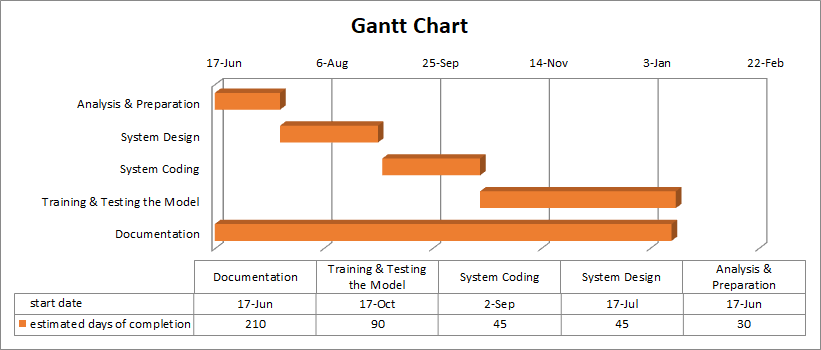
\includegraphics[width=6in]{images/gc2.png} 
	\caption{Gantt Chart} %figure name
	\label{figGanttChart} % for referencing
\end{center}
\end{figure}
\chapter{Literature Review}
\vspace{-18pt}
\section{Related Projects}
\vspace{-18pt}
\subsection{AI Stock Finder}
\vspace{-18pt}
It is a website that uses artificial intelligence algorithm to produce its forecasts based on 140 variables to yield high quality buy and sell signals. 
 \vspace{-10pt}
\subsection{Wallstreetzen Stock Forecast}
\vspace{-18pt}
WallStreetZen provides stock predictions and forecasts for the next 5 years. Their platform offers stock market forecasts for 2023, 2024, 2025, 2026, and 2027, along with analyst forecasts, price targets, buy/sell ratings, revenue/earnings forecasts, and more. Additionally, WallStreetZen offers a stock screener for identifying high-growth stocks based on analyst projections for the next 3 years . While it is important to note that stock market predictions and forecasts should be taken with caution, WallStreetZen provides a valuable tool for investors seeking insights into potential investment opportunities and market.
\vspace{-10pt}
\section{Related Works}
\vspace{-18pt}
Arjun Singh Saud and Subarna Shakya researched in detail about stock price prediction using different deep learning models. In the paper “Analysis of look back period for stock price prediction with RNN variants: A case study on banking sector of NEPSE” published on 2020, there is comparison of the predictions by the deep learning models used in the study: LSTM, VRNN and GRU. \cite{saud2020analysis}  Arjun Singh Saud and Subarna Shakya again in their paper "Analysis of Gradient Descent Optimization Techniques With Gated Recurrent Unit For Stock Price Prediction: A Case study on Banking Sector of Nepal Stock Exchange", have compared stock price prediction performance of GRU with three widely used gradient descent optimization techniques: Momentum, RMSProp, and Adam.\cite{saud2019analysis}  Nawa Raj Pokhrel, Keshab Raj Dahal, Ramchandra Rimal, Hum Nath Bhandari, Rajendra K.C Khatri, Binod Rimal and William Edward Hahn on their paper " Predicting NEPSE price index using deep learning models", have performed comparative analysis between the deep learning models on the basis of assessment metrics like Root Mean Square Error, Mean Absolute Percentage Error and Correlation Coefficient. \cite{pokhrel2022predicting}
\chapter{Methodology}
\vspace{-18pt}
  \section{Working Mechanism}
  \vspace{-18pt}
The development of stock price prediction system involves major steps which is 
depicted in the diagram given below:
\begin{figure}[tbh] % tbh means top, bottom or here (priority: left to right)
\begin{center}
	%
\includegraphics[width = 3in]{images/logo.png}
	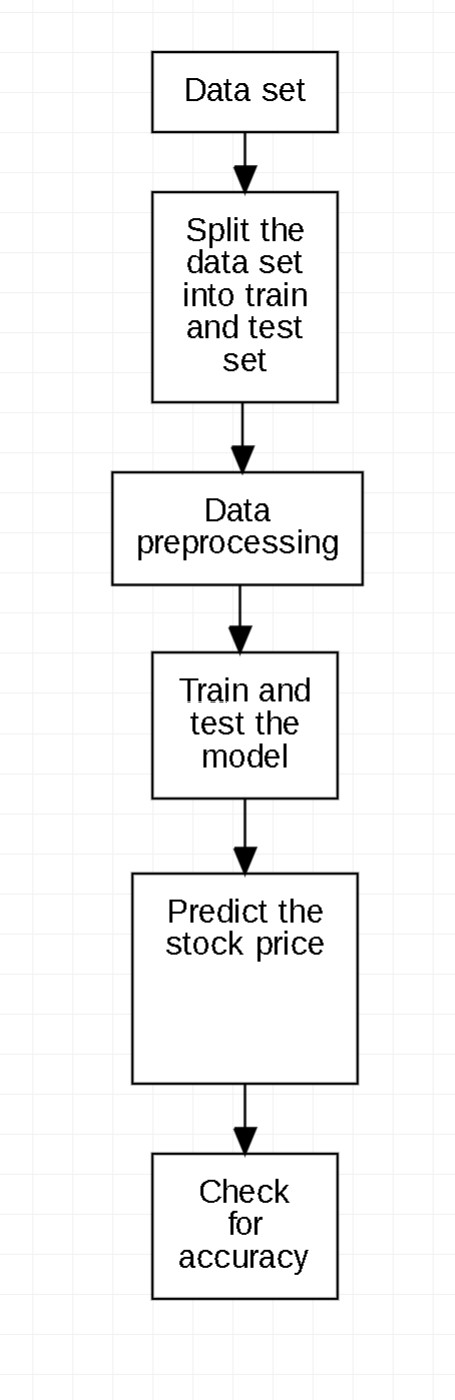
\includegraphics[width=2in]{images/wm.jpg} 
	\caption{Working mechanism of Stock Price Prediction System} %figure name
	\label{Working mechanism of Stock Price Prediction System} % for referencing
\end{center}
\end{figure}
\subsection{Data set}
\vspace{-18pt}
The data set contains financial data, macroeconomic data and technical indicators. Fundamental data is significant or historical data that provides important information needed for stock trading. It has an opening price, closing price, high price, low price and volume. The opening price is the first trading price at the opening of the trading day and the closing price is the last trading price of the stock that day. Likewise, the high and low prices are the highest and lowest prices for that day. Volume refers to the number of products traded in a trading day and indicates traders' interest in the market.High volume means more satisfaction and repetition. All business history data is daily data entry from Share Sansar portal, is one of the popular products providing detailed information about Nepal stock market.
\par
Macroeconomic data is a macroeconomic variable that affects stock market performance. Under the umbrella of macroeconomic factors, the representative features that affect stock price forecasts are remittances (RMT), inflation rate (IR), commercial bank interest rates (CBIR), treasury bills (TRB), consumer price index (CPI) and exchange rate (ER). Remittance is the money Nepalese workers send from abroad. Inflation is the rate of increase in prices over a given period of time.  The commercial bank interest rate is the bank rate at which Nepal Rastra Bank lends money to domestic financial institutions. The treasury bill is typically a promissory maturity note issued by a government as a primary instrument for regulating money supply and raising funds via open market operations. The Consumer Price Index is a measure of the average change overtime in the prices paid by urban consumers for a market basket of consumer goods and services. Exchange rate is the value of one country's currency against another country's currency.
 \par 
Technical indicator includes Moving Average Convergence Divergence (MACD), Average True Range (ATR), Relative Strength Index (RSI), and Money Flow Index (MFI). MACD is calculated by subtracting the 26-day exponential moving average (EMA) from the 12-day EMA. ATR measures the market volatility and is defined as follows:\newpage
\begin{eqnarray}
True Range(TR) = max{(H-L)|H-C_p|,|L-C_p|}\\
Average True Range(TR) = \frac{1}{n} \sum_{i}^{n}T R_i
\end{eqnarray}
where, H, L,$ C_p$ represent current high, current low, previous close prices and $T Ri, n$ represent a particular true range, the time period respectively.
\par 
The RSI is a momentum indicator that signals whether a security is overbought or oversold with current price levels, which is computed as follows:
\begin{equation}
RSI = 100 -\frac{100}{1 + \frac{Average Gain}{Average Loss}}
\end{equation}
where average gain and average loss are the average percentage gain and loss calculated over the certain look-back period.
\par 
The MFI communicates a possible reversal in time and provides a signal for further investment. Its calculation starts by finding the typical price (TP), the average of high, low, and close prices for each trading day. If the current TP is higher than the previous one, then positive money flow is calculated by multiplying the current TP with its volume. Similarly, a negative money flow is obtained if the current typical price is lower than the previous one. If the TP does not change, both positive and negative money flow will be zero. Summing all positive money flow indexes leads to positive money flow for a particular period. Negative money flow is calculated similarly. Mathematically, MFI is defined as: 
\begin{equation}
MFI = 100 - \frac{100}{1 + Money Ratio}
\end{equation}
\subsection{Split the data set into train set and test set}
\vspace{-18pt}
The data set is divided in train set and test set so that the train set can be used for training the model.
\subsection{Data Preprocessing}
\vspace{-18pt}
Data preprocessing consists of three major steps: Data cleaning, Feature selection and Time series analysis. Data cleaning includes removing or handling missing values, outliers, and errors in the data. This may involve techniques like imputation, interpolation, or removing problematic data points. Identifying the relevant features or variables that may affect stock prices. This could include factors like historical prices, trading volumes, technical indicators (e.g., moving averages, RSI), fundamental data (e.g., earnings, revenue), or macroeconomic indicators (e.g., interest rates, GDP) comes under Feature selection and Time series analysis consists of Techniques such as identifying trends, seasonality, or auto correlation can be applied to analyze and preprocess the data as stock price data is often represented as a time series. 
\subsection{Train the model}
\vspace{-18pt}
The models used in this project for stock price prediction are: Vanilla RNN (VRNN), Long Shortterm Memory (LSTM), and Gated Recurrent Unit (GRU).
\par 
\subsubsection{Long Short term Memory (LSTM)}
\vspace{-18pt}
LSTM is a popular deep learning technique in RNN for time series prediction. While standard RNNs outperform traditional networks in preserving information, they are not very effective in learning long term dependencies due to the vanishing gradient problem. An LSTM is well-suited to classify and/or predict time-series data. There are several architectures of LSTM units. A common architecture is composed of a memory cell, an input gate, an output gate and a forget gate. The mathematical formulation of the LSTM cell is given below:
\begin{eqnarray}
f_t = \sigma(x_tW_f + H_{t-1}U_f)\\
o_t = \sigma(x_tW_o + H_{t-1}U_o)\\
S_t = \sigma(S_{t-1} *f_t + i_t * H^{'}_t)\\
i_t = \sigma(x_tW_i + H_{t-1}U_i)\\
H^{'}_t = tanh(x_tW_g + H_{t-1}U_g)\\
H_t = tanh(S_t)*o_t
\end{eqnarray}
\begin{figure}[tbh] % tbh means top, bottom or here (priority: left to right)
\begin{center}
	%
\includegraphics[width = 3in]{images/logo.png}
	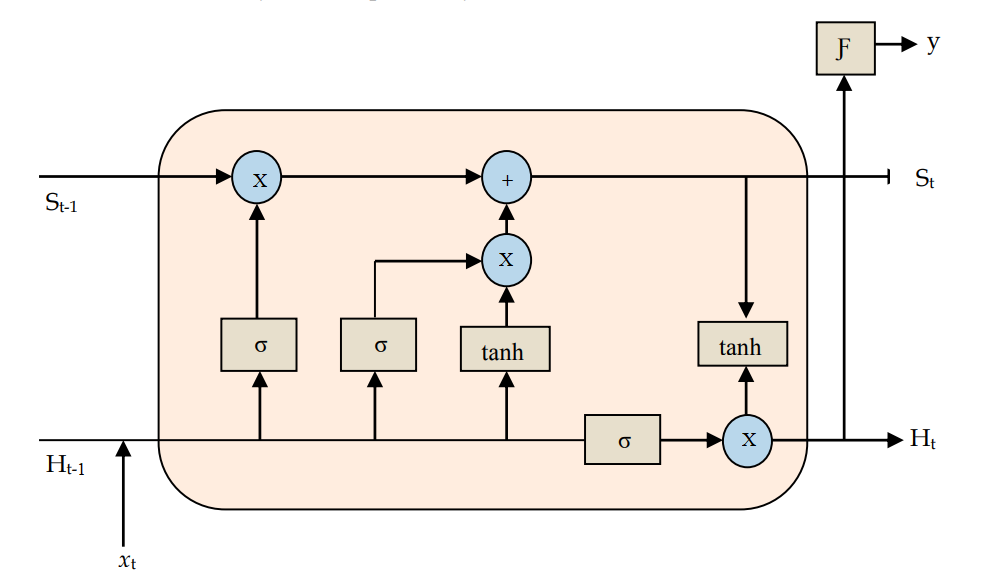
\includegraphics[width=6in]{images/l1.png} 
	\caption{LSTM} %figure name
	\label{LSTM} % for referencing
\end{center}
\end{figure}
\subsubsection{Vanilla RNN (VRNN)}
\vspace{-18pt}
It is the most basic form of a recurrent neural network. The simplest form of VRNN can be represented as in the figure given below. Normally, the tanh activation function is used in the hidden recurrent layer and the activation function for the output layer is selected according to the need of the problem to be solved. The operation of vanilla RNN can be expressed mathematically as below:
\begin{eqnarray}
H_t = f(W_{xh}X_t + W_{hh}H_{t-1})\\
O_t = g(W_{xo}S_t)
\end{eqnarray}
where $X_t$ is input at time t, $H_t$ is state info at time t, $W_{xh},W_{hh}$ and $W_{xo}$ are weight matrices.\newpage
\begin{figure}[tbh] % tbh means top, bottom or here (priority: left to right)
\begin{center}
	%
\includegraphics[width = 3in]{images/logo.png}
	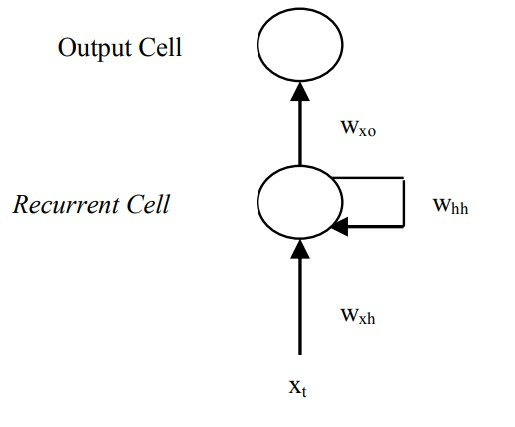
\includegraphics[width=4in]{images/vrnn.jpg} 
	\caption{VRNN} %figure name
	\label{VRNN} % for referencing
\end{center}
\end{figure}
\subsubsection{Gated Recurrent Unit Network}
\vspace{-18pt}
GRU is also a type of RNN architecture and aims to solve the vanishing gradient problem. GRU is similar to the LSTM but simplified in structure. GRU uses two gates: update gate and reset gate. The update gate of GRU is equivalent to the forget gate and input gate of LSTM. GRU has fewer parameters and thus may train faster. GRU cell takes two different pieces of information: the current input sequence $x_t$ , the short-term memory from the previous cell $H_{t-1}$, at time t. The update gate carries the long-term dependencies in GRU. It determines the past information that needs to be passed into the next step. The reset gate takes the information from $x_t$ and $H_{t-1}$ and produces the output between 0 and 1 through the sigmoid layer and then it identifies which information to discard from the previous hidden state $H_{t-1}$. When the value is 1, it stores all the information in the cell while with a value of 0, it forgets all the information from the previous hidden state. Based on empirical evidence, LSTM and GRU have proven their effectiveness on many machine learning tasks. The operation of GRU network can be expressed as follows: 
\begin{eqnarray}
Z_t = \sigma(W_zx_t + U_zH_{t-1})\\
H^{'}_t = tanh(W_hx_t + (R_t * H_{t-1})U_h)\\
R_t = \sigma(W_rx_t + U_rH_{t-1})\\
H_t = (Z_t*H^{'}_t)+((1-Z_t)*H_{t-1})
\end{eqnarray}
where Z and R are update and reset gates, and $H^{'}_t$ and $H_t$ are candidate hidden state and hidden states.
\begin{figure}[tbh] % tbh means top, bottom or here (priority: left to right)
\begin{center}
	%
\includegraphics[width = 3in]{images/logo.png}
	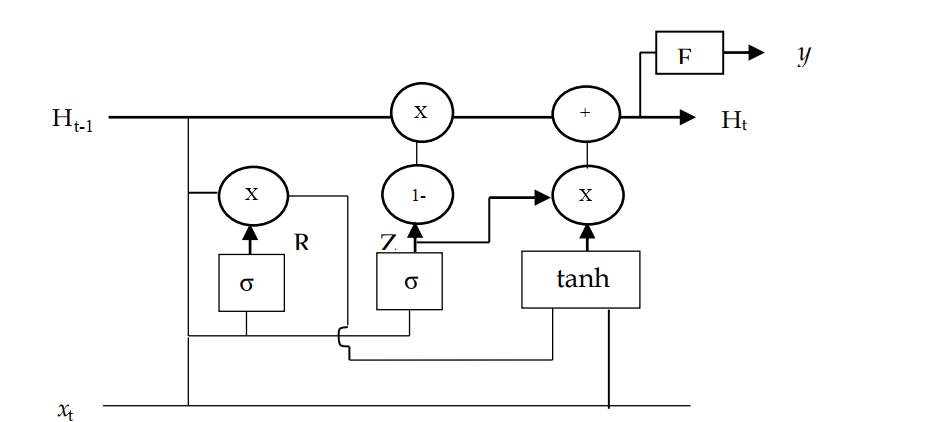
\includegraphics[width=5in]{images/gfig.png} 
	\caption{GRU network} %figure name
	\label{GRU network} % for referencing
\end{center}
\end{figure}
\subsection{Predict the stock price}
\vspace{-18pt}
Once the model is trained and evaluated, it can be used to make predictions on new, unseen data. This involves feeding the input features of the new data into the trained model, which then generates predictions for the corresponding stock prices.
\subsection{Check for accuracy}
\vspace{-18pt}
Mean Absolute Percentage Error (MAPE) is a measure of prediction accuracy in statistics. It is calculated as the average of the unsigned percentage error, which is the absolute value of the difference between the actual value and the forecast value divided by the actual value, multiplied by 100. The formula for Mean Absolute Percentage Error is given as:
\begin{equation}
M = \frac{1}{n} \sum_{t=1}^{n} | \frac{A_t - F_t}{A_t}|
\end{equation}
\section{System Diagram}
\vspace{-18pt}
\subsection{Use case diagram}
\begin{figure}[h]
\begin{center}
	%
\includegraphics[width = 3in]{images/logo.png}
	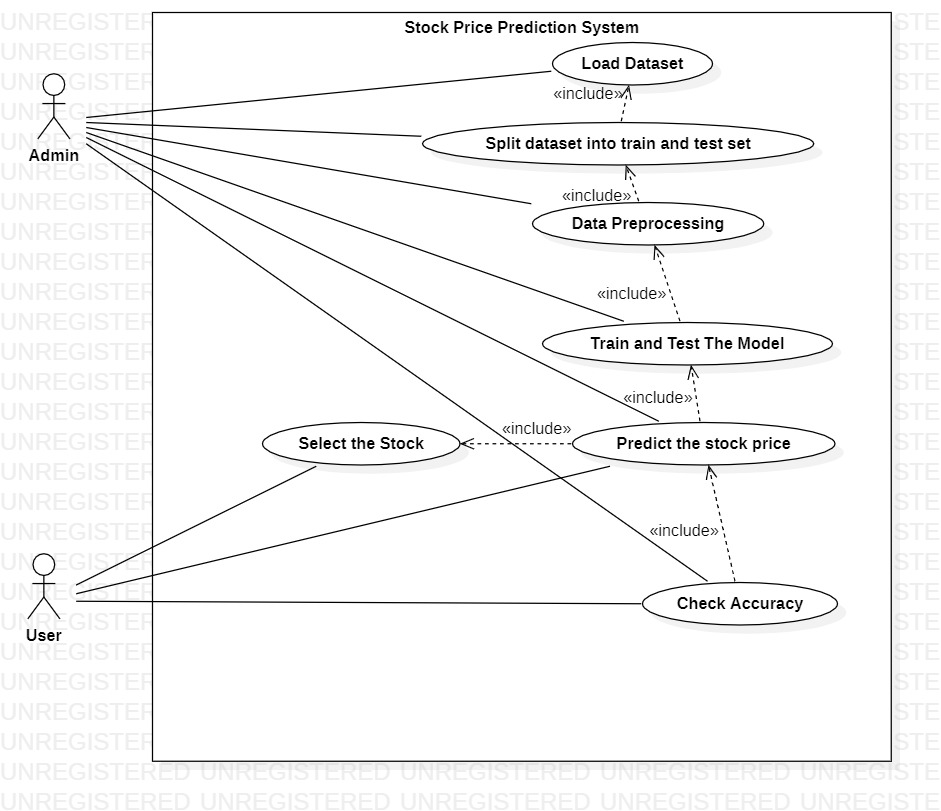
\includegraphics[width=5in]{images/ucd.jpg} 
	\caption{Use case Diagram of Stock Price Prediction System} %figure name
	\label{Use case Diagram of Stock Price Prediction System} % for referencing
\end{center}
\end{figure}
\newpage
\subsection{Software Development Model}
\vspace{-18pt}
 \begin{figure}[tbh] % tbh means top, bottom or here (priority: left to right)
\begin{center}
	%
\includegraphics[width = 3in]{images/logo.png}
	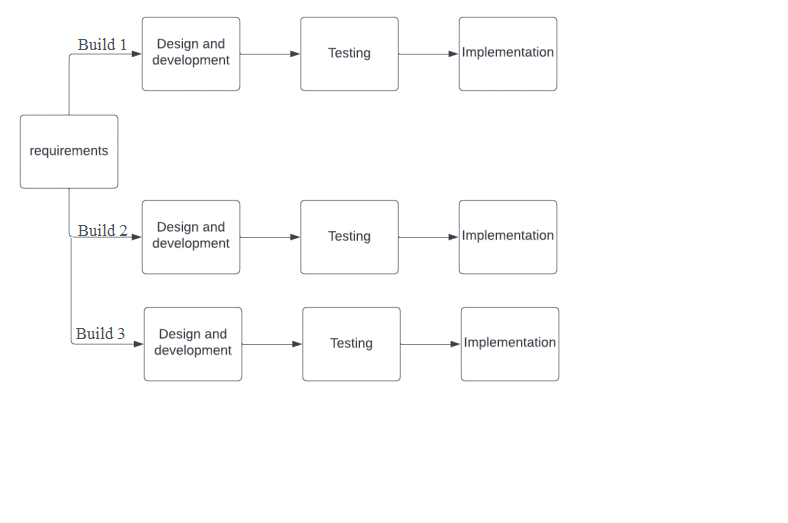
\includegraphics[width=8in]{images/sdlc1.png} 
	\caption{Incremental Model} %figure name
	\label{Incremental Model} % for referencing
\end{center}
\end{figure}
 Incremental model is a method of software engineering that combines the elements of waterfall model in iterative manner. It involves both development and maintenance. In this model requirements are broken down into multiple modules. Incremental development is done in steps from analysis design, implementation, testing/verification, maintenance. Each iteration passes through the requirements, design, coding and testing phases. The first increment is often a core product where the necessary requirements are addressed, and the extra features are added in the next increments. The core product is delivered to the client. Once the core product is analyzed by the client, there is plan development for the next increment.\\
\chapter{Epilogue}
\vspace{-18pt}
\section{Expected Output}
\vspace{-18pt}
Upon the completion of the project, the system will be able to predict the price of the stock the user selects.
%\chapter*{References}
%Reference
\renewcommand\bibname{REFERENCES} % Change heading to References
\bibliographystyle{IEEEtran} % to use IEEE Format for referencing
\addcontentsline{toc}{chapter}{References} % to add references in TOC
\bibliography{library} % specify the .bib file containing reference information 
\end{document}
